The main challenge, in this analysis, is to achieve reliable predictions of the low Standard Model background 
leading to the same-sign leptons + jets final state. 
This background is composed partly of rare processes such as the associate production of a top quark pair with a massive boson, 
or the production of multiple bosons. 
The other contribution consists in experimental backgrounds originating from the imperfect discrimination between prompt leptons and other objects, 
or the occasional misreconstruction of the electron charge. 
The following sections provide more details about the nature of these different categories of background, 
and the foreseen methods that will be used to estimate their contributions to the signal regions. 

\subsection{Backgrounds with prompt SS dilepton or three leptons}
\label{sec:bkg_prompt}

There are two main sources of Standard Model background leading to pairs of same-sign prompt leptons: 
\begin{itemize}
\item[$\bullet$] The associate production of top quark(s) and massive bosons, where the same-sign leptons pair 
is produced from leptonic decays of one of the top quarks and of the boson. 
These processes are characterized by a large jet multiplicity, the presence of $b$-jet(s), 
and always have intrinsic missing momentum. 
Therefore they generally represent the largest contribution to the signal regions. 
The dominant processes are $pp\to t\bar{t}W(j)$ and $pp\to t\bar{t}Z(j)$, 
while there are also minor contributions from $pp\to t\bar{t}H,\,tZbj,\,t\bar{t}WW$, and $pp\to t\bar{t}t\bar{t}$. 
\item[$\bullet$] The production of multiple massive bosons. 
These processes have generally low jet multiplicities. 
However, due to their larger cross-sections, they contribute in a significant way to the background entering signal regions without $b$-jets requirements. 
The dominant processes include $pp\to W^\pm W^\pm jj,\,WZ,\,ZZ$, 
with minor contributions from $pp\to\,WH,\,ZH,\,VVV$ and $pp \to\,H\to\,llll$.  
\end{itemize}

We plan to estimate the contributions of these various processes to the signal regions by relying on the Monte-Carlo predictions, 
normalized with the best known theoretical cross-sections : 
these processes are too rare to allow use of control regions until a significant integrated luminosity will be collected. 

Processes containing top quarks have cross-sections below 1~pb, which have consequently not yet been much constrained experimentally.
On the theoretical side, uncertainties on the cross sections are typically large: 30\% for $t\bar{t}W$ and 50\% for $t\bar{t}Z$
for the same-sign $\sqrt{s}=7$~TeV analysis~\cite{NoteSS3L_7TeV}, 22\% for both $t\bar{t}W$ and $t\bar{t}Z$ for the $\sqrt{s}=8$~TeV analysis~\cite{noteSS3L}. 

Cross-sections for diboson processes are known with a rather good accuracy, but only for the inclusive processes, 
while we are mostly interested in processes where several additional partons are produced. 

The validation regions described in section~\ref{sec:bkg_VR} will help us ensure that our understanding of these processes is sufficiently reliable, 
and that the systematic uncertainties assigned to the estimated rates are reasonable. 

\subsection{Charge flip leptons}
\label{sec:bkg_chflips}


Electrons are occasionally reconstructed with the wrong charge, 
generally because an irrelevant track is matched to the electron cluster during reconstruction instead of the real electron track. 
This may occur for example in the so-called trident process, where an electron emits a hard Brehmsstrahlung photon 
which further converts into an electron-positron pair, resulting in three close tracks. 
This confusion is the main reason for lepton charge flip, as errors on the track reconstruction itself are much rarer. 
Indeed, muon charge flip has been estimated negligible in past studies~\cite{noteSS3L}, and we consider only charge flip background originating from electrons. 

\begin{figure}[hbt]
\centering
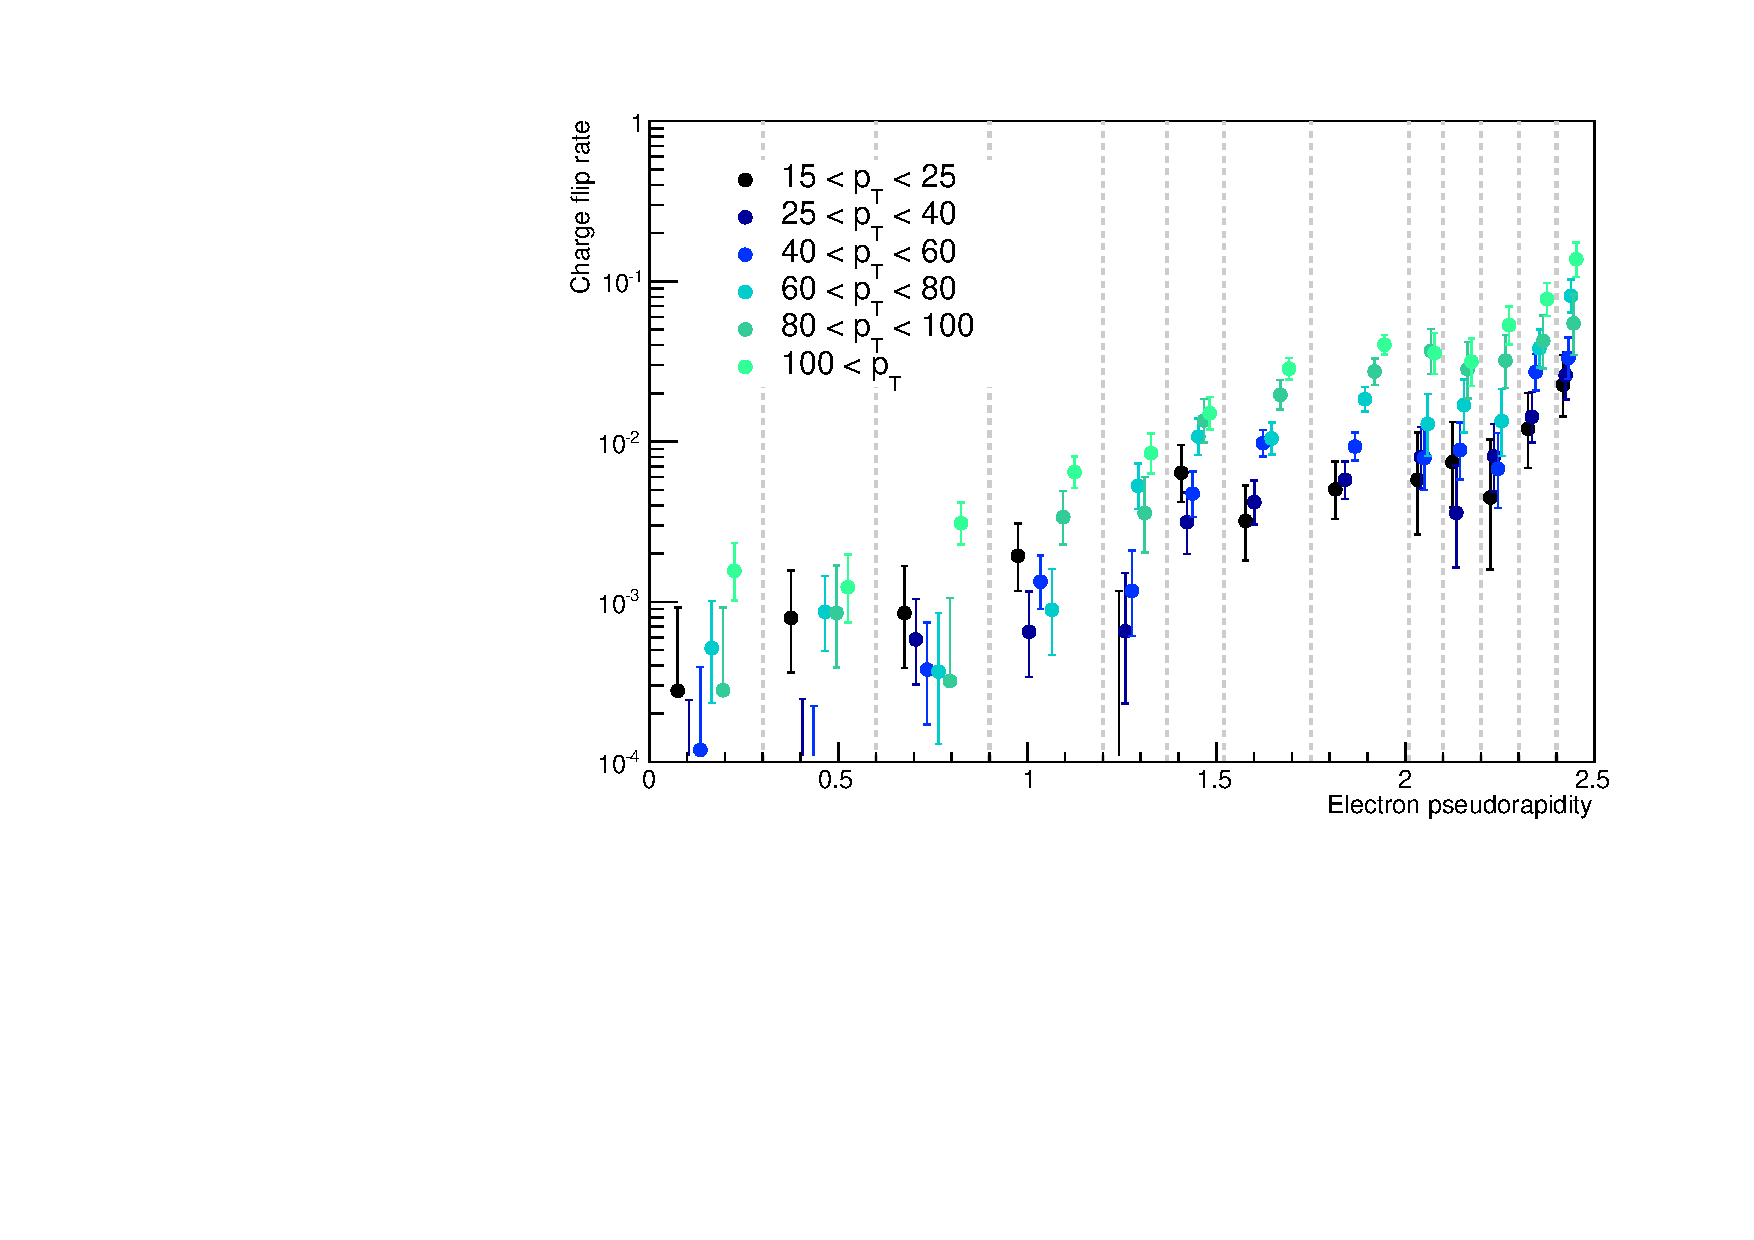
\includegraphics[width=0.7\textwidth]{BKG/chargeFlipRate}
\caption{Expected electron charge flip rate determined in simulated $t\bar{t}\to e\mu\nu\nu$ events}
\label{fig:mc_chargeflip_rate}
\end{figure}


This type of background is particularly relevant to searches with same-sign leptons, 
as they may turn a pair of opposite-sign leptons from an abundant Standard Model process ($pp\to Z,\,t\bar{t},\,W^+W^-$\ldots) 
into a much rarer same-sign pair.
Because of the jets requirements characteristic of our analysis, 
the dominant source of charge flip electrons in most of the signal regions arise from leptonic decays of $t\bar{t}$ pairs. 
This type of background contributes only moderately to the signal regions -- for example in the Run-1 analysis it represented at most 10\% of the total background yield. 
But for looser event selections, such as the ones used to validate the background modelling, it can be a major component in electron channels. 
It is therefore important to be able to predict reliably this background. 

Figure~\ref{fig:mc_chargeflip_rate} shows the expected rate of charge flip for electrons 
satisfying the requirements listed in sections~\ref{sec:objects_electrons} and~\ref{sec:isolation}, 
determined in simulated $t\bar{t}\to e\mu\nu\nu$ events. 
The rate increases significantly at large pseudorapidity, reflecting the larger amount of material in front of the calorimeter. 
There is also a significant dependency to the transverse momentum, with larger rates obtained for energetic electrons. 
\\
\par{\bf Background estimation methodology\\}
We rely on a purely data-driven method to estimate yields of events with charge flipped electrons. 
Assuming one knows the electron charge flip rates $\xi(\eta,p_T)$, a simple way to estimate the yields is to select 
events with pairs of opposite-sign leptons and assign them a weight: 

\begin{align}
w = \xi\left(\eta^{1},p_T^{1}\right)\left[1-\xi\left(\eta^{2},p_T^{2}\right)\right] 
+ \xi\left(\eta^{2},p_T^{2}\right)\left[1-\xi\left(\eta^{1},p_T^{1}\right)\right] 
\end{align}
where $\xi=0$ for muons. 

The advantages of this method are a good statistical precision since the charge flip rate is rather low, 
and the lack of dependency on the simulation and related uncertainties. 
Obviously, it requires a precise measurement of the rates, which is described in the next paragraph. 
Another inconvenient is that the reconstructed electron energy (hence momentum as well) of charge flipped electrons 
tends to be too low by a few~\GeV, because of the hard Brehmsstrahlung at the origin of the charge flip. 
Simply reweighting electrons from opposite-sign lepton pairs therefore does not predict correctly the charge-flip background shape 
for energy-dependent variables. 
In the past this effect was simply neglected, as we do not rely on discriminant variables very sensitive to the electron energy. 
But we are now considering applying energy correction factors, or assign dedicated systematic uncertainties. 
\\
\par{\bf Measurement of the charge flip rates\\}
The simulation of the charge flip process is not accurate enough to be relied on (discrepancies up to a factor 2 were seen in Run-1 analyses), 
therefore the rates have to be measured in data. 
In Run-2, electron charge flip rate measurements will be centralized by the Egamma performance group (unlike up to now). 
One of our group members is involved in these activities and will provide the rates according to our customized electron definitions. 
The standard method which will be employed for these measurements is similar to the one described 
in the documentation of the Run-1 same-sign leptons + jets search~\cite{noteSS3L}. 
It relies on the observed numbers of opposite (OS) and same-sign (SS) electrons with an invariant mass close to the $Z$ mass, 
which provides a clean sample of electrons. Expressing these numbers as function of the electron charge flip rate $\xi(\eta,p_T)$: 
\begin{align}
N_\text{SS}\left(\eta^{1},p_T^{1},\eta^{2},p_T^{2}\right) \approx 
\left[\xi\left(\eta^{1},p_T^{1}\right) + \xi\left(\eta^{2},p_T^{2}\right)\right] 
N\left(\eta^{1},p_T^{1},\eta^{2},p_T^{2}\right)\,,\quad N=N_\text{OS}+N_\text{SS}
\end{align}
the rates are then obtained as the maximum likelihood estimators for the product of Poisson distributions $\mathcal{P}(N_\text{SS}| N)$ 
binned in $\eta$ and $p_T$ of the two electrons. 

Sources of systematic uncertainties on the measured rates account for the background subtraction, 
and closure tests performed on Monte-Carlo (differences between the computed and true rates) 
and data ($Z$ lineshape opposite-sign electrons pairs reweighted by the measured rates, compared to the distribution of same-sign pairs). 

\subsection{Backgrounds with fake leptons}
\label{sec:bkg_fakes}

The term "fake lepton" denotes here any reconstructed lepton not originating 
from the decay of massive gauge or Higgs bosons, or an electroweak initial/final state radiation. 
They can be non-prompt leptons produced in heavy flavor meson decays, converted photons, 
light hadrons faking the electron shower, in-flight decays of kaons or pions to muons, etc.  
Common properties shared by these objects are a bad response to electron identification cuts, 
non-zero impact parameters, and the reconstructed leptons are often not well isolated; 
these properties can be used to discriminate fake leptons against the prompt leptons we are interested in. 

In signal regions enriched in $b$-jets, Monte-Carlo simulations predict that the dominant source of fake leptons originates 
from semileptonic $t\bar{t}$ events, with a non-prompt lepton in the decay chain of one of the $B$ mesons. 
Contributions from photon conversions and hadron fakes are not to be neglected though, 
in particular in $b$-jet-depleted signal regions where the rate of $t\bar{t}$ events is lower 
and is competed by processes such as $W\gamma$ + jets. 

We will rely on at least two different methods to estimate the fake leptons yields in the signal regions, 
which are briefly described in the next paragraphs. They have both been employed successfully in the Run-1 analysis~\cite{noteSS3L}. 

\subsubsection{The matrix method}
\label{sec:bkg_fakes_matrixmethod}

The matrix method is a purely data-driven approach 
which relies on the different response of prompt and fake leptons to identification, isolation and impact parameters requirements: 
fake leptons have low probabilities to satisfy these requirements, unlike prompt leptons. 
No tentative is made to consider the different categories of fake leptons separately -- systematic uncertainties are assigned in consequence. 
\\
\par{\bf Methodology\\}
A combination of tight requirements on discriminant variables such as electron identification, lepton isolation and impact parameters, is defined (see Tabe~\ref{tab:lepdef}). 
Reconstructed leptons are then classified in two categories ("tight" and "loose"), depending on their success satisfying the tight requirements or not. 
If $\epsilon$ and $\zeta$ are respectively the probabilities for a prompt/fake lepton to satisfy the requirements, 
linear relationships can be established between the mean values of the rates of prompt/fakes and tight/loose leptons, which for the 1-lepton case are: 
\begin{align}
\label{eqn:matrixmethod}
<N_\text{tight}> &= \epsilon <N_\text{prompt}> + \zeta <N_\text{fake}> \\\notag
<N_\text{loose}> &=  (1-\epsilon) <N_\text{prompt}> + (1-\zeta) <N_\text{fake}>
\end{align}

This system of equations can be used to evaluate the number of prompt and fake leptons given the observed number of tight and loose leptons. 
A detailed explanation of the generalization of the method to handle events with arbitrary number of leptons, as used in the Run-1 analysis, 
can be found in~\cite{noteSS3L,TomThesis}. 

The method relies of the prior knowledge of the probabilities $\epsilon$ and $\zeta$, 
which need to be measured in dedicated samples enriched in prompt and fake leptons (see next paragraph). 
The uncertainties on the probabilities for fake leptons constitute the main source of uncertainties in the asymptotic regime. 
In the low statistics regime, one has to cope with the fact that the loose and tight leptons categories are not enough populated 
to provide reliable estimates: 
for example predictions of negative yields are a possible outcome. 
In general these estimates are accompanied by large statistical uncertainties. 

Finally, one should note that the charge flip electron background interferes with the matrix method 
as charged flipped electrons are notably more prone to fail impact parameter or tight identification requirements, 
and the related efficiencies are distinct from both those of prompt and fake electrons. 
They correspond so to speak to a third category of objects, while the matrix method is based on the assumption that only two categories are present. 
One way to solve the issue is to rely on the linearity of the matrix method estimate with respect to its input number of events; 
therefore one can simply subtract the estimated charge flip background in the tight and loose leptons categories, from observed data. 
This requires a dedicated measurement of the charge flip rate for electrons failing the tight requirement. 
\\
\par{\bf Measurement of the $\epsilon,\zeta$ probabilities\\}
These parameters are measured in dedicated samples enriched in prompt or fake leptons. 
Probabilities for prompt leptons are measured in $Z\to \ell\ell$ tag-and-probe selections, 
and are assigned systematic uncertainties determined in Monte-Carlo covering the 
differences between the lepton properties in the measurement regions, 
and in the signal regions which have much busier event topologies. 
Other systematic uncertainties should account for the less isolated leptons that can be 
found in signal scenarios where decay products are particularly boosted (for example the gluino-stop offshell model). 

Probabilities for fake leptons are much harder to determine, due to the difficulty to identify 
an event selection that would provide both a high purity, and enough statistics, especially for leptons with $p_T>40$~\GeV. 
In the 8 TeV versions of this analysis, such selections were requiring at least two same-sign leptons together with a jet, 
and the fake electron probabilities were determined separately for events with or without $b$-jets. 
Other analyses have been using inclusive selections with a single lepton, 
which have the advantage to be much more populated, but on the other hand 
are less representative of the properties of fake leptons that can be found in our signal regions. 
In general the probabilities vary largely with $p_T$ (see e.g. the isolation efficiencies in section~\ref{sec:isolation}) thus require binned measurements. 

The measurements of fake leptons probabilities are associated to large uncertainties, 
which cover for the nature of the fake leptons and the events that produce them 
being different between the measurement and signal regions. 

\subsubsection{The Monte-Carlo template method}
\label{sec:bkg_fakes_mctemplates}

This method is Monte-Carlo based, and makes use of the samples corresponding to the various processes expected to produce fake leptons. 
Correction factors of the fake lepton modelling in the simulation are determined 
in a combined fit of several control regions involving shapes of discriminant variables such as the missing transverse momentum or the jet multiplicity. 
There are five such correction factors (for fake electrons and muons originating from light or heavy flavor jets, and an additional factor for charge flip), 
which are applied on an event basis depending on the generator information about the origin of the fake lepton in the event. 
More details can be found in the documentation of the Run-1 analysis~\cite{noteSS3L}. 

\subsubsection{Statistical tools improving robustness in low statistics regime}
\label{sec:bkg_fakes_stattools}

Some alternatives to the matrix method have been considered, based on the same principles but with more formal constructions as probabilistic tools 
(hence a better behaviour in conditions far from the asymptotic regime), and are currently being developed. 
One of these methods~\cite{PseudoLikelihoodMatrixMethod} relies on the construction of a likelihood function 
which translates the equation system~(\ref{eqn:matrixmethod}) in terms of probabilities for single leptons, instead of relationships between mean values; 
this also allows to treat $\epsilon$ and $\zeta$ as nuisance parameters (according to their measurements uncertainties) instead of being frozen. 
One could then simply estimate the rates of prompt and fake leptons as the maximum likelihood estimators of the observations, 
but the large number of parameters (several leptons per event hence many possible loose/tight combinations, binned probabilities $\epsilon$ and $\zeta$\ldots) 
renders this approach impractical. 
A simplification is discussed in~\cite{PseudoLikelihoodMatrixMethod,TomThesis}, which preserves some advantages over the standard matrix method. 

Another approach has been proposed recently~\cite{TomThesis}, 
consisting in building confidence intervals on the rate of fake leptons 
from the associated Bayesian posterior, which may be numerically computed with Gibbs sampling. 
The claimed advantages are a better assessment of the uncertainties on the final estimate, 
since the whole posterior distribution is known, 
as well as the absence of issues with local minima which might affect likelihood-based methods. 
More details can be found in~\cite{TomThesis}. 

We are planning to check if these methods can be applied with all the complexity of a real world analysis, 
in which case they would bring quite a nice improvement to the current way of predicting fake lepton background in the signal regions. 

\subsection{Backgrounds with fake $b$-jets}
\label{sec:bkg_bjetfakes}

In the signal regions requiring at least three $b$-jets, an important part of the background originates from processes 
with two real $b$-jets, and a third jet not originating from a $b$-quark but satisfying the $b$-tagging requirements. 
Unlike the case of fake leptons, the $b$-tagging performance group usually provides scale factors (and associated uncertainties) 
to correct the simulation for mismodelling both of real and fake $b$-jets. 
The fake leptons and charge flip background, being predicted from data, obviously do not need any correction. 

An alternative data-driven method was used in Run-1 as cross-check, 
consisting in the equivalent of the lepton matrix method but applying on jets 
and replacing lepton tight requirements by the output weight of the $b$-tagging algorithm. 
This approach was primarily developed for the ATLAS SUSY search with 0/1 lepton and 3 $b$-jets~\cite{SUSY3bjetsRun1}. 
It could be considered again for Run-2. 

\subsection{Neglected backgrounds}
\label{sec:bkg_neglected}
Other sources of background such as cosmic rays or cavern background, as well as pile-up events where two distinct proton-proton pairs may interact and produce leptons, 
have been evaluated in the past and found to be negligible. 
Multiple scattering effects are included in the simulations but are also not expected to contribute enough to require in-depth studies. 

\subsection{Validation regions}
\label{sec:bkg_VR}
The different type of backgrounds will be validated by looking at the agreement between the data observation and the SM expectation in regions dominated by one type of background. As for Run-1, several validation regions will be considered, and their definition is a balance between high purity, large statistics and low signal contamination. The latter is assured by requiring an upper cut on \met\ 
($<150$~\GeV). If no validation region can be designed, the background will be checked by looking at different kinematic variables distributions. For a complete validation, several selections will be considered :
\begin{itemize}
	\item{Loose: requiring at least two signal leptons in the event.}
	\item{Intermediate: adding soft cuts i.e. at least one or two signal jets or $b$ jets.}
	\item{Hard: increase the number of jets in the event.}
\end{itemize}


It is known that the associated uncertainty on the SM background can be decreased by adding control regions enriched in a certain type of background and orthogonal on the signal regions. However, given the rare SM processes which dominate in the signal regions, the statistics expected with $\sqrt s=$ 13 \TeV\ and $L$~$\le$3 \ifb of data in potential control regions is too small to be included. Hence, only validation regions will be defined for early Run-2.

\paragraph{\ttbar\ + $V$ background\\}
To validate the \ttbar\ + $Z$ and \ttbar\ + $W$ backgrounds estimation, several tentative regions defined with at least 1 or 2 $b$-jets in the event were considered. To decrease the other type of backgrounds, several jets and a low \met\ cut were also required. However, given the low statistics, it was found that a combined \ttbar~+~ $V$ region will perform better. The region definition is given in Table~\ref{tab:ttV_VR}. The leading and sub-leading leptons are required to be energetic (20 \GeV) in order to reduce the fake lepton background, while the veto on the fourth baseline lepton is minimizing the contamination from $ZZ$ processes. Note that it is very hard to obtain a pure validation region in \ttbar\ + $V$, as the difference with the other prompt SS SM processes is mainly the jet multiplicity. The highest purity was found when considering at least four jets in the $ee$ and $e\mu$ channels, and at least three jets in the $\mu\mu$ channel. A high \meff\ cut is used to further reduce the detector background, wile an upper cut of 900 \GeV\ is used to reduce the signal contamination. Note that this cut can be tighten to further decrease the SUSY contamination from models like direct sbottom. The reached purity for $\sqrt s=$ 13 \TeV\ and $L$~$\le$3 \ifb of data is around 42$\%$ if the large eta region is excluded ($|\eta|_e$~$<$~1.37) . The purity can be increased to 60$\%$ if the inclusive 1 $b$ jet selection is replaced by inclusive 2 $b$ jet selection (and the 400 \GeV\ cut on \meff\ is relaxed to 350 \GeV). The signal contamination was studied by looking at several available SUSY models studied in this analysis. It can be up to 27$\%$ when the direct-sbottom model is considered and the sbottom mass is 550 \GeV, or 20$\%$ for direct squark (2 step) via sleptons with $W/Z$ bosons in the cascade decay, otherwise it is smaller than 10$\%$. 

\begin{table}[htb!]
\caption{\ttbar\ + $V$ validation region definition. The \pt\ threshold of the leading two leptons is 20 \GeV, otherwise 10 \GeV.}
\label{tab:ttV_VR}
\begin{center}
    \begin{tabular}{|c|cc|c|c|}
      \hline
      \hline
     VR& $ N_{lept}^{signal}$ & $N_{lept}^{baseline}$ & $N_{b-jets}^{20}$     & Other variables \\ \hline
    ttV & $\ge 2$ &$<4$  & $\ge$1  & 30 $<$ \met $<$ 200 \GeV, 400 $<$ \meff $<$ 900 \GeV, $|\eta|_e$~$<$~1.37, \\
   &  & && $N_{jets}^{30}$ $\ge$ 4 in $ee$ and $e\mu$, $N_{jets}^{25}$ $\ge$ 3 in $\mu\mu$ channels\\	
      \hline
\end{tabular}
\end{center}
\end{table}


\paragraph{$ZZ$ + jets validation region\\}
Even if this type of background is minor in several of the defined signal regions, its contribution can is significant in regions with no $b$ jet requirement and three leptons. Therefore, a validation region was defined as presented in Table~\ref{tab:ZZ_VR}. It requires at least three signal leptons with \pt~$>$~20 \GeV, and at least four baseline leptons. The reached purity for $\sqrt s=$ 13 \TeV\ and $L$~$\le$3 \ifb of data is up to 97$\%$. In order to be closer to the SRs, another validation region can be defined by asking at least two jets with \pt~$>$~25 \GeV\ with a purity of 84$\%$. The signal contamination is at most 20$\%$.

\begin{table}[htb!]
\caption{$ZZ$ validation region definition. The \pt\ threshold of the two leading leptons is 20 \GeV, otherwise 10 \GeV. To be closer to the SRs, at least two jets with \pt~$>$~25 \GeV\ can be required in the event (and $N_{b-jets}^{20}$~$==$~0 becomes $N_{b-jets}^{20}$~$\ge$~0), without affecting the validation region purity.}
\label{tab:ZZ_VR}
\begin{center}
    \begin{tabular}{|c|cc|c|c|}
      \hline
      \hline
     VR & $ N_{lept}^{signal}$ & $N_{lept}^{baseline}$ & $N_{b-jets}^{20}$     & Other variables \\ \hline
     ZZ& $==3$ & $\geq 4$  & $==$0  & \met $<$ 150 \GeV, \meff $>$ 100 \GeV, $|\eta|_e$~$<$~2.  \\
     \hline
\end{tabular}
\end{center}
\end{table}


\paragraph{$WZ$ + jets validation region\\}
Similarly to $ZZ$ type of background, it is negligible in most of signal regions. However, it is expected to populate the regions with 0 $b$-jets and low jet multiplicity. Therefore, its validation is important and the proposed region definition is presented in Table~\ref{tab:WZ_VR}. It requires exactly three leptons and a veto on the fourth-leading baseline lepton in order to reduce the $ZZ$ background contamination. The lower cut on \met\ (30 \GeV) is mainly reducing the charge flip contamination. The \mt\ cut of 50 \GeV, even if is not used to define the signal regions, is assuring a smaller fake lepton contamination. At least one and at most three jets with \pt~$>$~25 \GeV are required in the event. It assures a purity of 70$\%$ for $\sqrt s=$ 13 \TeV\ and $L$~$\le$3 \ifb of data. The signal contamination is found to be below 1$\%$.

\begin{table}[htb!]
\caption{$WZ$ validation region definition. The \pt\ threshold of the two leading leptons is 20 \GeV, otherwise 10 \GeV.}
\label{tab:WZ_VR}
\begin{center}
    \begin{tabular}{|c|cc|c|c|}
      \hline
      \hline
     VR & $N_{lept}^{signal}$ & $N_{lept}^{baseline}$ &  $N_{b-jets}^{20}$     & Other variables \\ \hline
     WZ & $==$3 & $<4$  & $==$0  & 30 $<$ \met $<$ 300 \GeV, \mt~$>$50 \GeV, 1 $\leq$ $N_{jets}^{25}$ $\leq$ 3, $|\eta|_e$~$<$~2. \\
     \hline
\end{tabular}
\end{center}
\end{table}

\paragraph{$WW$ + jets validation region\\}
Similarly to the other diboson processes, the $WW$ + jets (with a pair of same sign lepton in the final state) events contribute mainly in the signal regions with no $b$ jet requirement. Two validation regions are defined (Table~\ref{tab:WW_VR}). In the first region, a cut on the invariant mass of the first two leading jets in the event is considered. It selects forward jets from VBS processes which are not necessary populating the signal regions defined in the analysis. However it is used as a cross-check as a high purity (50$\%$) can be reached. A second region is defined by selection two energetic jets (50 \GeV) and decreasing the electron acceptance to $|\eta|_e$~$<$~1.37. The purity is only 31$\%$. In both validation regions the signal contamination is at most 15$\%$.

\begin{table}[htb!]
\caption{$WW$ validation region definition. The \pt\ threshold of the two leading leptons is 20 \GeV.}
\label{tab:WW_VR}
\begin{center}
    \begin{tabular}{|c|cc|c|c|}
      \hline
      \hline
     VR & $N_{lept}^{signal}$ & $N_{lept}^{baseline}$ &  $N_{b-jets}^{20}$     & Other variables \\ \hline
     WW1 & $==$2 & $<3$  & $==$0  & 40 $<$ \met $<$ 300 \GeV, $Z$ mass veto,\\ 
     &&&& \mt~$>$40 \GeV, $N_{jets}^{40}$ $\ge$ 2, $m_{jj}$ $>$ 500 \GeV, $|\eta|_e$~$<$~2. \\\hline
     WW1 & $==$2 & $<3$  & $==$0  & 40 $<$ \met $<$ 300 \GeV, $Z$ mass veto,\\
     &&&& \mt~$>$40 \GeV, $N_{jets}^{50}$ $\ge$ 2, $|\eta|_e$~$<$~1.37 \\
     \hline
\end{tabular}
\end{center}
\end{table}

\paragraph{Fake lepton validation regions\\}
Beside the usual validation plots shown for the Run-1 analysis, several fake lepton validation regions are defined, in order to increase the confidence on the background estimation methods. Generally, depending on the $b$-jet multiplicity two categories are considered: low and high \meff, as presented in Table~\ref{tab:Fake_VR}. To reduce the charge flip background contamination, a veto on the $Z$ boson mass ($80<m_{\ell\ell}<100$~\GeV) is imposed only in the $ee$ channel. The background from prompt SS processes is reduced by a veto on the third baseline lepton. The leading two leptons are required to have a \pt\ threshold of 15 \GeV, and the event should have at least one jet. For the low \meff\ regions, the highest purity was reached when \met~$<$~100 \GeV\ and \meff~$<$~400 \GeV\ was imposed. A lower cut on \meff\ will drastically reduce the fake lepton background in the low \meff\ validation region, while in the high \meff\ region a higher threshold will increase the level of prompt SS background. Note that, the two validation regions overlap and the reached purity varies between 80 and 90$\%$. The signal contamination is found to be maximum 10$\%$.

\begin{table}[htb!]
\caption{Fake lepton validation region definition. The \pt\ threshold of the two leading leptons is 15 \GeV. }
\label{tab:Fake_VR}
\begin{center}
    \begin{tabular}{|c|cc|c|c|}
      \hline
      \hline
      \multicolumn{5}{|c|}{\textbf{Low meff fake leptons VRs}}\\
      \hline
      \hline
     VR & $N_{lept}^{signal}$ & $N_{lept}^{baseline}$ & $N_{b-jets}^{20}$     & Other variables \\ \hline
     FL0b-L\meff& $==$2 & $<3$  & $==$0  & 20 $<$ \met $<$ 100 \GeV, \meff $<$ 400 \GeV, \mt~$<$60 \GeV, $N_{jets}^{25}\geq 1$ \\
     FL1b-L\meff& $==$2 & $<3$  & $==$1  & 20 $<$ \met $<$ 100 \GeV, \meff $<$ 400 \GeV, \mt~$<$60 \GeV\\
     FL2b-L\meff&$==$2  & $<3$ & $\ge$2  & 20 $<$ \met $<$ 100 \GeV, \meff $<$ 400 \GeV, \mt~$<$80 \GeV \\
     \hline
      \hline
      \multicolumn{5}{|c|}{\textbf{High meff fake leptons VRs}}\\
      \hline
      \hline
     VR & $N_{lept}^{signal}$ & $N_{lept}^{baseline}$ & $N_{b-jets}^{20}$     & Other variables \\ \hline
     FL0b-H\meff& $==$2 & $<3$ & $==$0  & 20 $<$ \met $<$ 100 \GeV, \meff $>$ 300 \GeV, \mt~$<$100 \GeV, $N_{jets}^{25}\geq 1$ \\
     FL1b-H\meff& $==$2 & $<3$ & $==$1  & 20 $<$ \met $<$ 50 \GeV, \meff $>$ 300 \GeV, \mt~$<$80 \GeV\\
     FL2b-H\meff&$==$2  & $<3$ & $\ge$2  & 20 $<$ \met $<$ 50 \GeV, \meff $>$ 300 \GeV, \mt~$<$50 \GeV\\
     \hline
\end{tabular}
\end{center}
\end{table}


